\documentclass[aspectratio=169]{beamer}
\usetheme{uantwerpen}

\usepackage{mathtools}

% tikz
\usepackage{tikz}
\usetikzlibrary{automata,positioning,overlay-beamer-styles}

% macros
\newcommand{\always}{\mathop{\mathtt{G}}}
\newcommand{\evtly}{\mathop{\mathtt{F}}}
\newcommand{\until}{\mathrel{\mathtt{U}}}
\newcommand{\nxt}{\mathop{\mathtt{X}}}

% titlepage info
\title{Acacia-Bonsai}
\subtitle{A Modern Implementation of Downset-Based LTL Synthesis}
\author{Micha\"el Cadilhac \and \underline{Guillermo A. P\'erez}}
\date{TACAS 2023}

% outline before each section
\AtBeginSection[]
{
  \begin{frame}
    \frametitle{Outline}
    \tableofcontents[currentsection]
  \end{frame}
}

\begin{document}

\begin{frame}
	\titlepage
\end{frame}

\begin{frame}{Motivation: Safe Reactive Systems}
  \begin{block}{Reactive systems}
    These are systems that interact with their environment in a
    \alert{continuous} fashion, i.e. nonstop, and they are all around us:
    e.g. operating systems, schedulers, embedded controllers\dots
  \end{block}
  \begin{center}
    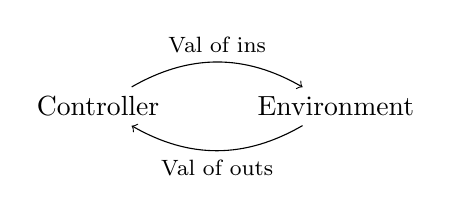
\begin{tikzpicture}
      \node (cnt) {Controller};
      \node[right= of cnt] (env) {Environment};
      \path[->,auto]
        (cnt) edge[bend left] node{\footnotesize Val of ins} (env)
        (env) edge[bend left] node{\footnotesize Val of outs} (cnt)
        ;
    \end{tikzpicture}
  \end{center}
  \pause
  \begin{block}{Safety via synthesis}
    Reactive systems are hard to design and errors can \alert{cost lives} and
    money. Hence, we would like to \alert{synthesize them} from a formal
    specification!
  \end{block}
\end{frame}

\begin{frame}{Motivation: Synthesis Competition}
  \begin{block}{SYNTCOMP}
    Since 2014, the synthesis competition SYNTCOMP gathers benchmarks and
    tools for synthesis from different specification formats:
    \begin{itemize}
      \item Safety monitors
      \item \alert{Linear temporal logic (LTL) formulas}
      \item Parity games
    \end{itemize}
  \end{block}
  \pause
  \begin{block}{LTL syntesis tools}
    Award winning tools include:
    \begin{itemize}
      \item Strix
      \item ltlsynt
      \item \alert{Acacia (no longer maintained)}
      \item \dots
    \end{itemize}
  \end{block}
\end{frame}

\section{LTL Specifications}

\begin{frame}{Linear temporal logic}
  \begin{block}{Formulas}
    Fix a set $P$ of \alert{atomic propositions}. LTL formulas are of the
    form:
    \[
      \varphi \Coloneqq a \in P \mid \varphi \land \varphi \mid
      \lnot \varphi \mid \nxt \varphi \mid \evtly \varphi \mid
      \always \varphi \mid \varphi \until \varphi
    \]
  \end{block}

  \begin{block}{Why LTL?}
    It allows to naturally specify time dependence amongst events.
    It has applicaitons in:
    \begin{itemize}
      \item Artificial intelligence
      \item Hybrid systems and control
      \item Software engineering
      \item Bio-informatics
      \item \dots
    \end{itemize}
    It forms the basis of the \alert{Property Specification Language} (IEEE
    1850) that can be used with electronic system design languages (HDLs e.g.
    Verilog).
  \end{block}
\end{frame}

\begin{frame}{Semantics of LTL}
  \begin{block}{Semantics over words (by example)}
    ``It is always the case that if there is a request then eventually it is
    granted'':
    \[ \varphi = \bigwedge_{i=1,2} \always(\mathit{req}_i \rightarrow \evtly
    \mathit{grant}_i)\]
    \begin{itemize}
      \item
        $(\mathit{req}_1,\mathit{req}_2,\mathit{grant}_1,\overline{\mathit{grant}_2})^*
        (\overline{\mathit{req}_1},\overline{\mathit{req}_2},\overline{\mathit{grant}_1},\mathit{grant}_2)^\omega$
        \alert{satisfies} $\varphi$
        \pause
      \item
        $(\overline{\mathit{req}_1},\overline{\mathit{req}_2},\mathit{grant}_1,\mathit{grant}_2)^\omega
        \models \varphi$
    \end{itemize}
  \end{block}
  \pause
  \begin{block}{The synthesis problem}
    Does there exist a \alert{controller} $\sigma : Val(ins)^* \to Val(outs)$
    such that all outcomes consistent with $\sigma$ satisfy the specification?
    \pause
    \begin{itemize}
      \item For $\varphi$ as above, with $ins = \{req_i\}$ and $outs = \{grant_i\}$,
        \alert{yes!} ``grant all requests immediately''
    \end{itemize}
  \end{block}
\end{frame}

\section{Synthesis Algorithms}

\begin{frame}{Classical Algorithms}
  \begin{center}
    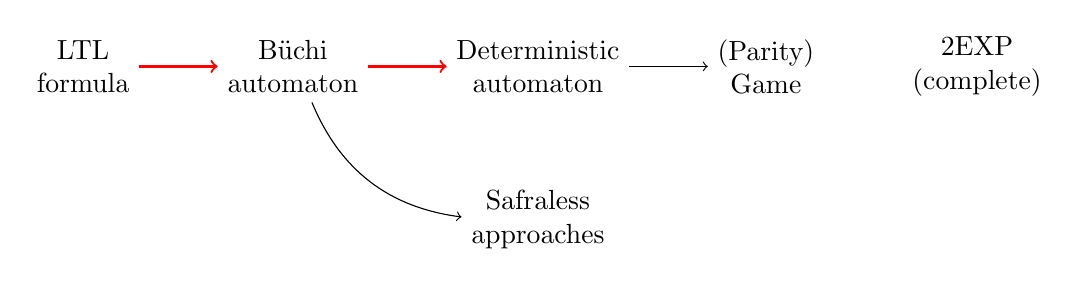
\begin{tikzpicture}
      \node[align=center] (spec) {LTL\\formula};
      \node[right= of spec,align=center] (auto) {B\"uchi\\automaton};
      \node[right= of auto,align=center] (det) {Deterministic\\automaton};
      \node[right= of det,align=center] (game) {(Parity)\\Game};
      \node[right= of game,align=center] {\alert{2EXP}\\\alert{(complete)}};
      \node[below= of det,align=center,visible on=<3->] (safraless)
        {Safraless\\approaches};
      \path[->]
        (spec) edge[thick,color=red] (auto)
        (auto) edge[thick,color=red] (det)
        (det) edge (game)
      ;
      \path[->,visible on=<3->]
        (auto) edge[bend right] (safraless)
      ;
    \end{tikzpicture}
  \end{center}
  \visible<2->{
    \begin{block}{Important optimizations}
      \begin{itemize}
        \item Normalization procedures on the LTL formula
        \item On-the-fly construction of the deterministic automaton (and game)
        \item \dots
      \end{itemize}
    \end{block}
  }
\end{frame}

% 4. Safety approximation: to avoid determinization
\begin{frame}{From LTL to B\"uchi Automata: Example}
  \[ \lnot\left(\bigwedge_{i=1,2} \always(\mathit{req}_i \rightarrow \evtly
  \mathit{grant}_i)\right)\]
  %
  \pause
  %
  \begin{center}
    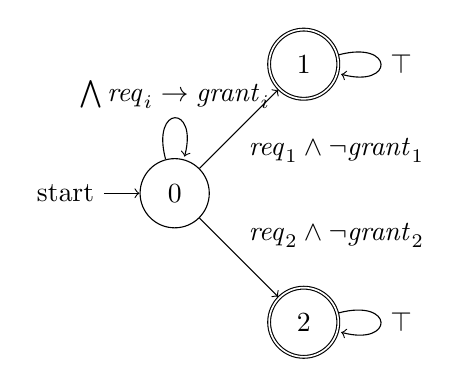
\begin{tikzpicture}
      \node[initial,state](s0){0};
      \node[state,accepting,above right= of s0](s1){1};
      \node[state,accepting,below right= of s0](s2){2};
      \path[->,auto]
        (s0) edge[loop above] node{$
          \bigwedge \mathit{req}_i \rightarrow \mathit{grant}_i
        $} (s0)
        (s0) edge node[swap]{$\mathit{req}_1 \land \lnot \mathit{grant}_1$} (s1)
        (s0) edge node{$\mathit{req}_2 \land \lnot \mathit{grant}_2$} (s2)
        (s1) edge[loop right] node{$\top$} (s1)
        (s2) edge[loop right] node{$\top$} (s2)
      ;
    \end{tikzpicture}
  \end{center}
\end{frame}

\begin{frame}{Let's Play a Game}
  \begin{block}{The synthesis game}
    Let $\mathcal{A}_{\lnot \varphi}$ be the B\"uchi automaton for the
    complement of the specification $\varphi$. In each round of the game:
    \begin{enumerate}
      \item Environment chooses a valuation of ins,
      \item Controller then chooses a valuation of outs.
    \end{enumerate}
    The (infinite) outcome is \alert{winning for Controller} iff it
    satisfies $\varphi$ iff it is \emph{not} accepted by $\mathcal{A}_{\lnot
    \varphi}$.
    \begin{itemize}
      \item Non-determinism in $\mathcal{A}_{\lnot \varphi}$ makes things
        algorithmically difficult\dots
    \end{itemize}
  \end{block}
  \pause
  \begin{block}{A handicapped game}
  \end{block}
\end{frame}

\section{Downsets}
% 5. Downsets (a.k.a. Antichains)

\section{Acacia-Bonsai and Experiments}
% 6. Tool architecture and features
% 7. Experimental results

\section{Conclusion}
% 8. Conclusion + future work

\end{document}
